% --------------------------------------------------------------------------
% DCASE 2026 Workshop paper — Task 7 (Domain-Incremental Learning for Audio
% Classification).
% To be used with:
%   dcase2026.sty  - DCASE 2026 workshop LaTeX style file, and
%   IEEEtran.bst   - IEEE bibliography style file.
% --------------------------------------------------------------------------

\documentclass[9pt,conference]{IEEEtran}
\usepackage{dcase2026}
\usepackage{bm}
\usepackage{amsmath,graphicx,url,times,booktabs,tabularx}

% Example definitions.
% --------------------
\def\defeqn{\stackrel{\triangle}{=}}
\newcommand{\symvec}[1]{{\mbox{\boldmath $#1$}}}
\newcommand{\symmat}[1]{{\mbox{\boldmath $#1$}}}

% Title.
% --------------------
\title{PER-DOMAIN RESIDUAL ADAPTERS WITH ASYMMETRIC DEPTH FOR\\
DOMAIN-INCREMENTAL AUDIO CLASSIFICATION}

\name{Aakash Divakar*, Angad Ripudaman Singh Bajwa*, Atharva Anand Joshi*\thanks{*The three authors
contributed equally to this work.}}
\address{Independent Researcher, Austin, USA \\
         \{aakashdivakar.4869, angadisthere, atharvajoshi253\}@gmail.com}

\begin{document}
\maketitle
\sloppy

\begin{abstract}
We describe our submission to DCASE 2026 Task~7, Domain-Incremental
Learning (DIL) for audio classification, where a system ranked 5th on the
challenge leaderboard. Starting from the released ADIL baseline, which adds
per-domain Batch Normalization (BN) and a per-domain classifier to a shared,
frozen CNN14 backbone, we identify limited per-domain capacity as the main
bottleneck on the harder domains. We insert, on top of the frozen backbone,
a stack of zero-initialised \emph{residual bottleneck adapters} after every
convolutional block. Because each domain owns an independent adapter stack,
its depth can be set \emph{per domain}: the harder domain (D3) receives a
deeper stack than the easier one (D2). Combined with a warm-started
per-domain classifier head and a supervised contrastive auxiliary loss, this
raises the domain-agnostic average accuracy on the dev-test set from
$50.0\%$ to $68.5\%$, with D2 and D3 improving from $59.2\%/40.8\%$ to
$76.2\%/60.8\%$. We further study three domain-routing strategies and a
waveform-augmentation pipeline, and show that a lightweight learned router
can add a further $0.8$ points on dev-test but generalises poorly to the
unlabeled evaluation set, whereas the parameter-free entropy router remains
the more robust choice. Finally, we stress-test the system on ESC-50, a
domain never seen during training: accuracy on the overlapping classes is
higher than on the in-domain dev-test references, but entropy routing
confidently misroutes this genuinely unseen audio rather than abstaining,
which we identify as a more practical failure mode than raw accuracy. The
shared backbone and D1 behaviour are preserved bit-for-bit, so no
previously learned domain is forgotten.
\end{abstract}

\begin{IEEEkeywords}
Domain-incremental learning, continual learning, acoustic
classification, residual adapters, catastrophic forgetting
\end{IEEEkeywords}


\section{Introduction}
\label{sec:intro}

Domain-incremental learning (DIL) requires a single model to classify the
same set of sound classes as the recording conditions change over a
sequence of domains $\mathcal{D}_1 \rightarrow \mathcal{D}_2 \rightarrow
\mathcal{D}_3$, without access to the data of previous domains and without
forgetting them \cite{mulimani2025dil}. Naively fine-tuning the whole
network on a new domain overwrites the knowledge of earlier domains
(catastrophic forgetting), while freezing the network entirely prevents it
from adapting (poor plasticity). This stability-plasticity trade-off is
shared with the broader continual-learning literature, but DIL differs from
class-incremental learning in that the label space is fixed and only the
acoustic conditions shift, and from unsupervised domain adaptation in that
no source data is available once a new domain arrives.

The DCASE 2026 Task~7 baseline addresses this trade-off with the ADIL
approach \cite{mulimani2025dil}: a CNN14 \cite{kong2020panns} backbone is
trained on $\mathcal{D}_1$ and then \emph{frozen}; for every subsequent
domain only a small set of domain-specific parameters is learned, namely
the affine Batch-Normalization (BN) parameters of that domain and a
residual correction to the classifier. At inference the domain identity is
not given, so the model forward-passes through every domain's specific
layers and selects the domain whose prediction has the lowest entropy
(domain-agnostic, ADIL).

This design forgets nothing, because the parameters of earlier domains are
never touched, but its plasticity is limited: a handful of affine BN
parameters is often too little capacity to absorb a large distribution
shift, which is exactly what we observe on the two harder development
domains, where the reproduced baseline reaches only $59.2\%$ (D2) and
$40.8\%$ (D3). Adapter modules that add a small number of task-specific
parameters to an otherwise frozen backbone are a natural way to increase
plasticity without disturbing previously learned weights, and have been
used extensively for efficient transfer in NLP and vision; here we adapt
this idea to the DIL, forgetting-free setting of Task~7. The contribution
of this report is to \emph{increase the per-domain capacity} while keeping
the forgetting-free property intact (Fig.~\ref{fig:arch}). Specifically, we
(1) add per-domain residual bottleneck adapters after every convolutional
block, (2) make the adapter depth \emph{asymmetric}, giving the harder
domain more capacity than the easier one, (3) replace the shared classifier
with a warm-started per-domain head, (4) tighten the per-class embedding
clusters with a supervised contrastive loss, and (5) compare three
domain-routing strategies at inference time. All additions are per-domain
and zero/identity-initialised, so $\mathcal{D}_1$ is reproduced exactly and
the domains remain mutually independent. The resulting system placed 5th
in the DCASE 2026 Task~7 challenge; this paper reports the full ablation
and routing study behind that submission.


\section{Method}
\label{sec:method}

\begin{figure*}[t]
  \centering
  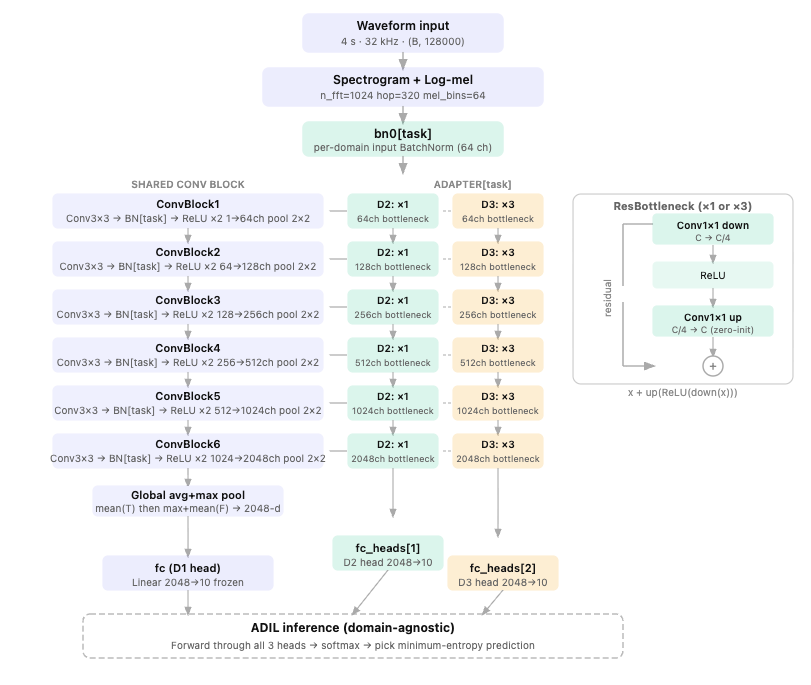
\includegraphics[width=0.68\textwidth]{Dcase_task7_architecture.png}
  \caption{Architecture of the submitted system. A shared, frozen CNN14
    backbone (purple) is augmented with per-domain components: an input and
    per-block Batch Normalization, a stack of zero-initialised residual
    bottleneck adapters after every convolutional block (green for D2,
    amber for D3, with asymmetric depth $1$ vs.\ $3$), and a per-domain
    linear head. At inference the input is routed through all domains and
    the minimum-entropy prediction is kept (ADIL). The inset details one
    residual bottleneck adapter.}
  \label{fig:arch}
\end{figure*}

\subsection{Backbone and per-domain Batch Normalization}
\label{ssec:backbone}

We keep the baseline front-end and backbone unchanged. Audio is resampled
to $32$~kHz; a log-mel spectrogram with $64$ mel bands is computed with a
window of $1024$ and a hop of $320$ samples. The backbone is CNN14
\cite{kong2020panns}: six convolutional blocks producing
$\{64,128,256,512,1024,2048\}$ channels, each block being two $3\times3$
convolutions, each followed by BN and ReLU, and a $2\times2$ average
pooling. Following the baseline, the convolutional weights are loaded from
the released $\mathcal{D}_1$ checkpoint and \emph{frozen for all domains};
only the BN layers are made domain-specific, i.e.\ each domain $t$ owns its
own BN parameters and statistics.

\subsection{Per-domain residual bottleneck adapters}
\label{ssec:adapters}

To give each domain more than the affine BN capacity, we insert a residual
bottleneck adapter after each of the six convolutional blocks. For a
feature map with $C$ channels the adapter is
\begin{equation}
  \label{eqn:adapter}
  \mathrm{Adapter}(\symvec{x}) =
    \symvec{x} + W_{\text{up}}\,\sigma\!\big(W_{\text{down}}\,\symvec{x}\big),
\end{equation}
where $W_{\text{down}}$ is a $1\times1$ convolution reducing the channels
to $C/4$, $\sigma$ is a ReLU, and $W_{\text{up}}$ is a $1\times1$
convolution restoring $C$ channels. $W_{\text{up}}$ is
\emph{zero-initialised}, so at the start of training every adapter is the
identity map and the pretrained features are left untouched; the adapter
then learns a domain-specific feature shift on top of the frozen backbone.
Domain $\mathcal{D}_1$ uses identity adapters, so its behaviour is
reproduced bit-for-bit.

\subsection{Asymmetric adapter depth}
\label{ssec:asym}

Because each domain owns an independent stack of adapters, the
\emph{number} of adapters stacked after each block can be chosen per
domain. We stack $d_t$ residual adapters for domain $t$:
\begin{equation}
  \label{eqn:stack}
  \mathrm{Stack}_t(\symvec{x}) =
    \big(\mathrm{Adapter}^{(d_t)} \circ \cdots \circ
         \mathrm{Adapter}^{(1)}\big)(\symvec{x}).
\end{equation}
Every adapter in the stack is zero-initialised, so a stack of any depth
still starts as the identity. We set $d_{\mathrm{D2}}=1$ and
$d_{\mathrm{D3}}=3$: the harder domain D3 receives three times the
per-domain convolutional capacity of D2. Since the two stacks are
completely independent, increasing D3's depth cannot affect D2.

\subsection{Per-domain classifier head}
\label{ssec:head}

The baseline reuses the frozen $\mathcal{D}_1$ classifier for all domains.
We instead give every domain $t>0$ its own linear head
$\symvec{W}_t\in\mathbb{R}^{C\times K}$ ($K=10$ classes), warm-started from
the $\mathcal{D}_1$ classifier at checkpoint-load time. $\mathcal{D}_1$
keeps the original head. The head is trained jointly with the domain's BN
and adapters.

\subsection{Training objective}
\label{ssec:loss}

Each domain is trained with cross-entropy plus a supervised contrastive
auxiliary loss \cite{khosla2020supcon} applied to the L2-normalised global
embedding $\symvec{z}$:
\begin{equation}
  \label{eqn:supcon}
  \mathcal{L}_{\mathrm{con}} =
    \sum_{i}\frac{-1}{|P(i)|}\sum_{p\in P(i)}
      \log\frac{\exp(\symvec{z}_i\!\cdot\!\symvec{z}_p/\tau)}
               {\sum_{a\neq i}\exp(\symvec{z}_i\!\cdot\!\symvec{z}_a/\tau)},
\end{equation}
where $P(i)$ is the set of samples sharing $i$'s class. The total loss is
$\mathcal{L} = \mathcal{L}_{\mathrm{CE}} +
\lambda\,\mathcal{L}_{\mathrm{con}}$ with $\lambda=0.2$ and $\tau=0.07$,
which pulls same-class embeddings together and pushes different-class
embeddings apart, sharpening the per-domain decision boundaries.

\subsection{Waveform-level data augmentation}
\label{ssec:data_aug}
We additionally evaluated a training-only waveform augmentation pipeline
(validation/test loaders stay deterministic). Each 4~s training segment
keeps one unmodified view plus, by default, eight augmented views with a
random composition of conservative transforms: temporal (zero-filled time
shift, stretch, speed, fade); class-aware pitch/tempo shifting with
narrower ranges for tonal/speaker-like classes (piano, speech) than
texture-like ones (engine, footsteps), to avoid flipping the label; spectral
filtering and additive colored noise ($18$--$35$~dB SNR); a low-level,
label-preserving distractor clip mixed in at $8$--$20$~dB SNR; and local
corruption (temporal masking, gain perturbation, mild soft clipping). The
waveform is re-cropped/padded and peak-normalised only if its peak exceeds
one.

\subsection{Domain routing at inference}
\label{ssec:routing}

Since the domain identity of a test sample is unknown, we need a routing
rule that selects which domain-specific layers to use. We compare three
strategies on top of the same trained model.

\noindent\textbf{Entropy routing.} The baseline strategy requires no
additional training. For each test sample we compute class probabilities
under each domain head, $\mathbf{p}_t = \mathrm{softmax}(\mathbf{l}_t)$,
and select the domain with minimum predictive entropy
\cite{mulimani2025dil}:
\begin{equation}
  \label{eqn:entropy_routing}
  t^* = \arg\min_{t}\; H_t, \qquad
  H_t = -\sum_{c} p_{tc}\log p_{tc}.
\end{equation}
A well-matched domain head produces a peakier, lower-entropy distribution
than a mismatched one, so $t^*$ acts as an implicit domain detector; this
mirrors how predictive entropy is used for confidence estimation in deep
ensembles \cite{lakshminarayanan2017ensembles}.

\noindent\textbf{Mahalanobis distance router.} Following Lee et al.\
\cite{lee2018mahalanobis}, we model each domain's distribution in the
D1-BN feature space $\mathbf{z}=g_0(\mathbf{x})\in\mathbb{R}^{2048}$ (the
GAP output of Conv~Block~6 under frozen D1 statistics). From the D2 and D3
training embeddings we estimate diagonal-covariance Gaussians
$(\boldsymbol{\mu}_k,\boldsymbol{\Sigma}_k)$ with a $\lambda=10^{-4}$
diagonal regulariser via streaming statistics, and route by
\begin{equation}
  \label{eqn:mahal_routing}
  t^* = \begin{cases}
    D1 & \text{if } \min(d_{D2},\,d_{D3}) > \tau, \\
    \arg\min_k\; d_k(\mathbf{z}) & \text{otherwise,}
  \end{cases}
\end{equation}
with $d_k(\mathbf{z})=\sqrt{(\mathbf{z}-\boldsymbol{\mu}_k)^\top
\boldsymbol{\Sigma}_k^{-1}(\mathbf{z}-\boldsymbol{\mu}_k)}$ and a rejection
threshold $\tau=60$ calibrated on dev-test, below which a sample is routed
to D1 instead of D2/D3.

\noindent\textbf{GAP-MLP router.} As a learned alternative, in the spirit
of mixture-of-experts gating \cite{jacobs1991moe,fedus2022switch}, we
concatenate the domain-specific GAP activations from all three heads
($3\times2048=6144$-d) and train a Linear($6144\!\to\!256$)-ReLU-Linear
($256\!\to\!2$) MLP with cross-entropy on the labeled development split
(Adam, 5~epochs, $\mathrm{lr}=10^{-3}$) to predict $\{D2,D3\}$; a sample is
rejected to D1 if $\max(\mathrm{softmax})<\tau_{\mathrm{MLP}}=0.5$.

Unless noted otherwise, the submitted system uses entropy routing, which
adds zero parameters and requires no domain labels at any stage.


\section{Experiments and results}
\label{sec:results}

\subsection{Setup}
\label{ssec:setup}

All systems are trained on the Task~7 development set, one domain at a
time, starting from the released $\mathcal{D}_1$ checkpoint. We use Adam
with learning rate $10^{-3}$, batch size $32$, and a CosineAnnealingLR
schedule decaying to $10^{-7}$. Only the current domain's parameters (BN,
adapters, head) are updated at each step. We report the domain-agnostic
accuracy on D2 and D3, and their average, after the full
$\mathcal{D}_1\!\rightarrow\!\mathcal{D}_2\!\rightarrow\!\mathcal{D}_3$
sequence, on the dev-test split (D2: 639 samples, D3: 806 samples). The
submitted configuration trains for 180~epochs with $\lambda_{con}=0.2$,
$\tau=0.07$, and asymmetric depths $(1,3)$; the augmentation experiment
(Sec.~\ref{ssec:aug_results}) uses the same setting for 240~epochs with
waveform augmentation enabled.

\subsection{Ablation}
\label{ssec:ablation}

Table~\ref{tab:ablation} adds one component at a time. Residual adapters
give the largest single jump ($+13.7$ average over the BN baseline),
confirming that per-domain capacity, not the classifier, is the
bottleneck. The per-domain head and the contrastive loss mainly help D2,
while the asymmetric depth and longer training are what move the harder D3
domain (from $55.1\%$ to $60.8\%$). The submitted system reaches $68.5\%$
average, an $18.5$-point improvement over the reproduced baseline, while
preserving D1 exactly.

\begin{table}[t]
  \centering
  \caption{Domain-agnostic accuracy ($\%$) on the dev-test split, adding
           one component at a time. The last row is the submitted system.}
  \label{tab:ablation}
  \begin{tabularx}{\columnwidth}{Xccc}
    \toprule
    System & D2 & D3 & Avg \\
    \midrule
    Per-domain BN (baseline) \cite{mulimani2025dil} & 59.2 & 40.8 & 50.0 \\
    \;+ residual adapters            & 73.9 & 53.5 & 63.7 \\
    \;+ per-domain head              & 77.3 & 54.0 & 65.6 \\
    \;+ supervised contrastive loss  & 77.9 & 55.1 & 66.5 \\
    \;+ asymmetric depth (1,\,3)     & 77.2 & 57.7 & 67.4 \\
    \;+ longer training (180 ep.)    & \textbf{76.2} & \textbf{60.8} & \textbf{68.5} \\
    \bottomrule
  \end{tabularx}
\end{table}

\subsection{Choosing the adapter}
\label{ssec:adapter_choice}

Before settling on residual bottleneck adapters we compared three
per-domain adapter families inserted at the same six locations, each
trained under the identical protocol (Table~\ref{tab:adapter}).
Feature-wise linear modulation (FiLM), which only scales and shifts each
channel, performed \emph{below} the BN baseline: a per-channel affine
transform is too weak to absorb the distribution shift. Squeeze-and-
excitation (SE) channel gating helped ($57.7\%$), but stacking more SE
blocks did not. The residual bottleneck, which mixes channels through its
$1\times1$ convolutions, was clearly the strongest ($63.7\%$) and is the
one we keep. The gap is largest on the harder D3 domain
($38.8\rightarrow53.5\%$), confirming that the bottleneck's extra capacity
is what the difficult domain needs.

\begin{table}[t]
  \centering
  \caption{Per-domain adapter family, same backbone and protocol
           (residual bottleneck selected).}
  \label{tab:adapter}
  \begin{tabularx}{\columnwidth}{Xccc}
    \toprule
    Adapter family & D2 & D3 & Avg \\
    \midrule
    FiLM (affine per channel)        & 56.7 & 38.8 & 47.7 \\
    Squeeze-and-excitation           & 70.3 & 45.0 & 57.7 \\
    Squeeze-and-excitation (deeper)  & 69.2 & 41.8 & 55.5 \\
    Residual bottleneck (\emph{ours}) & \textbf{73.9} & \textbf{53.5} & \textbf{63.7} \\
    \bottomrule
  \end{tabularx}
\end{table}

\subsection{Domain routing strategies}
\label{ssec:routing_results}

Table~\ref{tab:routing} compares all three routing strategies on top of
the best single model (\texttt{bn\_res\_deep\_clf}, asymmetric depth
$1,3$, 180~epochs).

\begin{table}[t]
  \centering
  \caption{Routing strategy comparison on the dev-test split.}
  \label{tab:routing}
  \begin{tabularx}{\columnwidth}{Xccc}
    \toprule
    Router & D2 & D3 & Avg \\
    \midrule
    Entropy (no threshold)         & \textbf{76.2} & 60.8 & 68.5 \\
    Entropy + ensemble ($\times$2) & 74.0 & 50.5 & 60.9 \\
    Mahal.\ (no threshold)         & 70.9 & \textbf{62.5} & 66.7 \\
    Mahal.\ ($\tau=60$, diag)      & 68.5 & 57.7 & 63.8 \\
    GAP-MLP (3~ep., $\tau_{\text{MLP}}=0.5$) & 76.5 & 62.0 & \textbf{69.3} \\
    \bottomrule
  \end{tabularx}
\end{table}

Entropy routing works well with no training overhead, and benefits
implicitly from the per-domain head calibration enforced by the supervised
contrastive loss: well-calibrated heads produce more separable entropy
values across domains. Mahalanobis routing adds an explicit geometric
model of the domain feature distributions. Without a rejection threshold
it matches entropy routing in final accuracy ($66.7\%$) while achieving
$73.2\%$ D2$\leftrightarrow$D3 routing accuracy on dev-test, confirming
that D2 and D3 occupy separable, though overlapping, regions in D1-BN
space (mean distances $d_{D2}\!\approx\!42.0$, $d_{D3}\!\approx\!44.0$).
With $\tau=60$, $22.8\%$ of D2/D3 samples are rejected to D1, which
\emph{degrades} average accuracy: a global distance threshold is a coarse
instrument when the D1 and D2/D3 distributions are not cleanly separated.

GAP-MLP routing concatenates domain-specific GAP representations from all
three heads. The best epoch (3) reaches $69.3\%$ average accuracy on
dev-test but overfits quickly: epoch 5 degrades D2 from $76.5\%$ to
$75.0\%$ and the average from $69.3\%$ to $68.9\%$. More tellingly, on the
\emph{unlabeled} evaluation set the learned router assigns only $0.6\%$ of
samples to D1 ($61.0\%$/$38.5\%$ to D2/D3) — it almost never rejects a
sample, suggesting it memorised the dev-train distribution rather than a
robust rejection criterion. We keep entropy routing as the submitted
default: GAP-MLP and Mahalanobis show that a well-calibrated single model
already captures most of the achievable routing accuracy here, while
learned routers add a threshold-calibration burden without a reliable
held-out gain.

\subsection{Effect of waveform augmentation}
\label{ssec:aug_results}
Table~\ref{tab:augmentation} reports the result of enabling the
waveform-level augmentation pipeline (Sec.~\ref{ssec:data_aug}), trained
for $240$ epochs with the same $\lambda_{con}=0.2$, $\tau=0.07$, and
asymmetric depths $(1,3)$ as the submitted system.

\begin{table}[t]
  \centering
  \caption{Waveform augmentation result.}
  \label{tab:augmentation}
  \begin{tabularx}{\columnwidth}{Xccc}
    \toprule
    System & D2 & D3 & Avg \\
    \midrule
    waveform augmentation
      & 75.4 & 51.4 & 63.4 \\
    \bottomrule
  \end{tabularx}
\end{table}

The augmented run remains strong on D2 but loses accuracy on D3 relative
to the best non-augmented asymmetric-depth system. This suggests the
augmentation distribution may be too broad for the hardest domain: while
the perturbations improve diversity, aggressive temporal warping, pitch
changes, filtering, and distractor mixing can also move some samples away
from the D3 characteristics that the adapter stack needs to specialise
for. We therefore treat this pipeline as a robustness-oriented ablation
rather than the final selected configuration; test-time augmentation and
checkpoint ensembling were likewise within noise of the single frozen
model and were dropped to keep the submission simple.

\subsection{Asymmetric depth and contrastive weight}
\label{ssec:choices}

Giving \emph{both} domains depth-2 stacks scored $65.1\%$, whereas the
asymmetric $(1,3)$ allocation reached $67.4\%$ at a similar parameter
budget: the capacity is better spent on the domain that actually needs it
(D3) than spread evenly. Sweeping the SupCon weight
$\lambda\in\{0.1,0.15,0.2,0.25,0.3\}$ peaked at $\lambda=0.2$ ($66.7\%$);
larger values began to compete with the cross-entropy term and slightly
hurt accuracy.

\subsection{Frozen backbone vs.\ partial unfreezing}
\label{ssec:discussion}

The most tempting way to gain more D3 accuracy is to unfreeze the top
convolutional blocks of the shared backbone (Table~\ref{tab:unfreeze}).
Unfreezing two blocks for D3 \emph{does} push D3 as high as $66.4\%$ ---
the best D3 number we obtained --- but because the backbone is shared, D2
collapses to $58.5\%$, since D2's BN and adapters were tuned for the
original features. Anchoring the drift with an $\ell_2$ penalty toward the
previous checkpoint recovers D2 but cancels most of the D3 gain, and
restricting the unfreezing to D3's own forward pass still leaves D2
degraded. Unfreezing three blocks destabilises training entirely. Across
the whole sweep, \emph{no} unfrozen configuration beat the fully-frozen
adapter system on average: the shared weights couple the domains and trade
one against the other. We therefore keep the backbone frozen and rely on
per-domain adapters, which add plasticity \emph{without} any cross-domain
interference.

\begin{table}[t]
  \centering
  \caption{Partial backbone unfreezing for D3. No configuration beats the
           frozen adapter system; the shared weights couple D2 and D3.}
  \label{tab:unfreeze}
  \begin{tabularx}{\columnwidth}{Xccc}
    \toprule
    Configuration & D2 & D3 & Avg \\
    \midrule
    Frozen adapters (submitted)        & \textbf{76.2} & 60.8 & \textbf{68.5} \\
    Unfreeze 2 blk, no anchor          & 58.5 & \textbf{66.4} & 62.5 \\
    Unfreeze 2 blk, $\ell_2$ anchor    & 75.3 & 57.3 & 66.3 \\
    Unfreeze 1 blk, $\ell_2$ anchor    & 72.6 & 57.7 & 65.2 \\
    D3-only unfreeze 2 blk             & 61.5 & 62.3 & 61.9 \\
    D3-only unfreeze 3 blk             & 46.3 & 54.3 & 50.3 \\
    \bottomrule
  \end{tabularx}
\end{table}

\subsection{Generalization to an unseen domain}
\label{ssec:esc50}

To probe generalisation beyond $\mathcal{D}_1$--$\mathcal{D}_3$, we run the
submitted system, \emph{with no further training}, on ESC-50
\cite{piczak2015esc50}, recorded on entirely different sources and
microphones. We use the 7 ESC-50 categories overlapping the Task~7 label
space (alarm, baby\_cry, dog\_bark, engine, fire, footsteps, knocking;
$40$ clips/class), and compare against a matched $40$-clip/class subsample
of the same 7 classes from D2/D3 dev-test.

\begin{table}[t]
  \centering
  \caption{Accuracy and routing on an unseen domain (ESC-50) vs.\
           class-balanced in-domain references (7 classes, 40 clips/class).}
  \label{tab:esc50}
  \begin{tabularx}{\columnwidth}{Xccc}
    \toprule
    Test set & Acc.\,(\%) & Mean $H$ & D1/D2/D3 (\%) \\
    \midrule
    ESC-50 (unseen)   & 85.0 & 0.027 & 14/53/33 \\
    D2 dev-test (ref.) & 71.9 & 0.060 & 14/54/32 \\
    D3 dev-test (ref.) & 55.7 & 0.027 & 19/34/47 \\
    \bottomrule
  \end{tabularx}
\end{table}

Two findings stand out. Accuracy on unseen ESC-50 clips is \emph{higher}
than on either in-domain reference, so the D2/D3 gap is not simply domain
novelty: ESC-50's single-source, high-SNR recordings are acoustically
easier, and part of the D3 shortfall in Table~\ref{tab:ablation} is
intrinsic sample difficulty rather than insufficient adapter capacity.
More importantly, entropy routing has no notion of ``none of the above'':
ESC-50 is routed to D2/D3 with mean entropy ($0.027$) as low as the
confident D3 reference. A router calibrated only on
$\mathcal{D}_1$--$\mathcal{D}_3$ will confidently mis-route out-of-scope
audio rather than abstain; only an explicit-rejection router, e.g.\
thresholded Mahalanobis distance (Sec.~\ref{ssec:routing}), can express
``this is neither D2 nor D3,'' which we see as the more practical failure
mode to address before deployment.


\section{Conclusion}
\label{sec:conclusion}

We presented a forgetting-free extension of the DCASE 2026 Task~7 baseline
that increases per-domain capacity through zero-initialised residual
adapters, with asymmetric depth, a warm-started per-domain classifier, and
a supervised contrastive loss. The system raises the domain-agnostic
dev-test average from $50.0\%$ to $68.5\%$ while reproducing
$\mathcal{D}_1$ exactly, and placed 5th in the DCASE 2026 Task~7 challenge.
Entropy routing remains the most robust of the three routers studied: it
needs no training and, unlike GAP-MLP, does not overfit to the labeled
split or misroute unseen-domain audio with false confidence (Sec.~\ref{ssec:esc50}).
Closing the D3 gap without the cross-domain interference seen when
unfreezing the backbone, and combining entropy routing's reliability with
an explicit rejection option, are left for future work.


% -------------------------------------------------------------------------
\bibliographystyle{IEEEtran}
\bibliography{refs}

\end{document}
